\documentclass{ximera}

\title{Concavity and Graphing Activity Solution Guide }
\author{MATH 425: Calculus I}

\begin{document}
\begin{abstract}
   Working with the peers in your group, solve the following problems. Make sure to show and justify all your work. Make sure everyone in the group understands the solution and participates. Be prepared to report your answers to the whole class. 
\end{abstract}
\maketitle


\begin{exercise}
    The following graph is the graph of the derivative $f'$ of a function $f$.  Use the information from the first derivative to sketch a graph of $f$. (Your graph should include what you know about increasing, decreasing, concave up and concave down.)\\
    \begin{image} 
        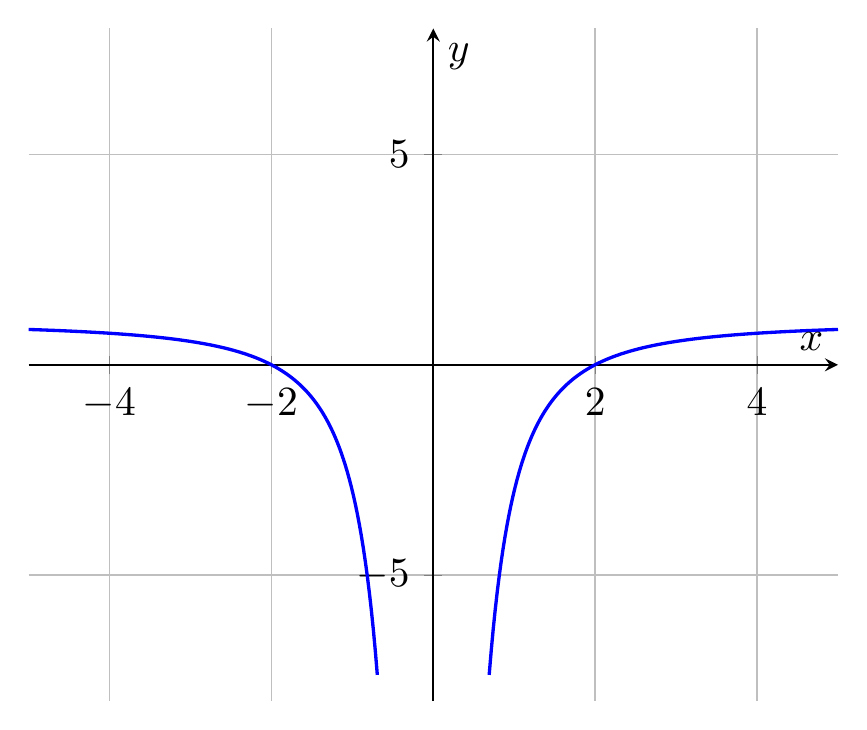
\begin{tikzpicture}[scale=1.5]
            \begin{axis}[
                axis lines=middle,
                grid=major,
                xmin=-5, xmax=5,
                ymin=-8, ymax=8,
                xlabel=$x$,
                ylabel=$y$,
                samples=200,
                restrict y to domain=-8:8,
               % discontinuities={-0.01, 0.01}
            ]
                \addplot[blue, thick, domain=-5:-0.1]{(x^2-4)/x^2};
                \addplot[blue, thick, domain=0.1:5]{(x^2-4)/x^2};
                
                % Vertical asymptote at x=0
                %\addplot[dashed, gray]{x/x * NaN};
                %\draw[dashed, gray] (0,-8) -- (0,8);
                
                % Horizontal asymptote at y=1
                %\draw[dashed, gray] (-5,1) -- (5,1);
            \end{axis}
        \end{tikzpicture}
    \end{image}
    \textcolor{blue}{The graph of $f$ should be increasing on $(-\infty,-2)$ and $(2,\infty)$ and decreasing on $(-2,0)$ and $(0,2)$.  The graph of $f$ should be concave up on $(-\infty,0)$ and concave down on $(0,\infty)$.  
    \begin{image} 
        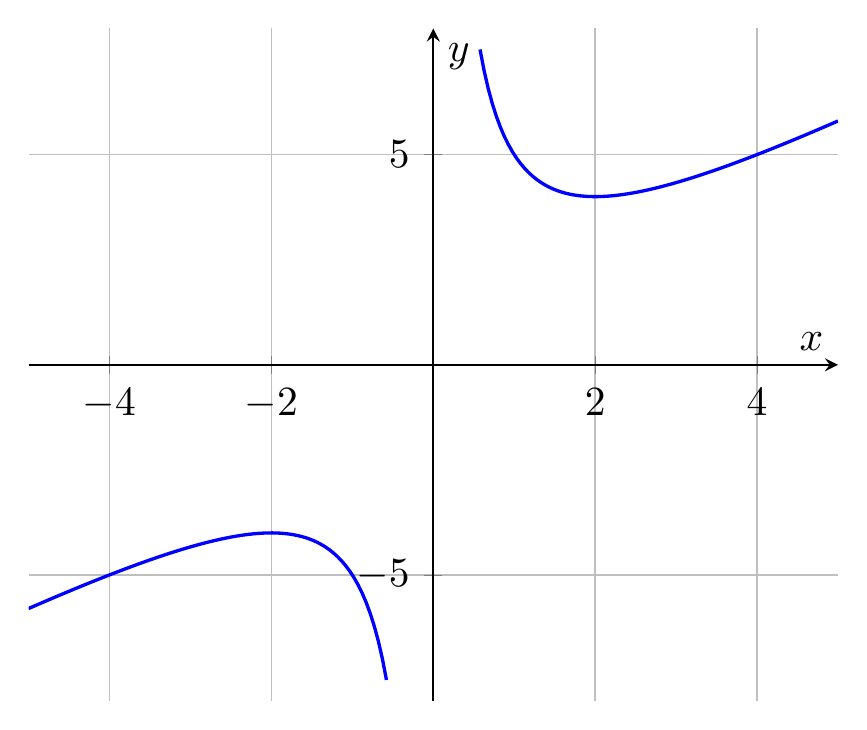
\begin{tikzpicture}[scale=1.5]
            \begin{axis}[
                axis lines=middle,
                grid=major,
                xmin=-5, xmax=5,
                ymin=-8, ymax=8,
                xlabel=$x$,
                ylabel=$y$,
                samples=200,
                restrict y to domain=-8:8
            ]
                \addplot[blue, thick, domain=-5:5]{x+4/x};
            \end{axis}
        \end{tikzpicture}
    \end{image}
    }
\end{exercise}

\begin{exercise}
    Sketch the graph of a function $g(x)$ that satisfies all of the following conditions: \\
    \begin{tabular}{c|c|c|c}
       Interval  & $g$ & $g'$ & $g''$  \\ \hline
        $(-\infty, -1)$ &  & $g'(x)>0$ & $g''(x)>0$\\
        x=-1 & 0 & DNE & DNE \\
        $(-1, 3)$ & & $g'(x)<0$ & $g''(x)>0$\\
        x=3 & -3 & 0 & $g''(x)>0$\\
        $(3,5)$ & & $g'(x)>0$ & $g''(x)>0$\\
        x=5 & 4 & $g'(x)>0 $& 0\\
        $(5,\infty)$ & & $g'(x)>0$ & $g''(x)<0$
    \end{tabular}
    \textcolor{blue}{This is one example of many that would work for this function:
    \begin{image}
        
\includegraphics{Concavity2a.jpg}
    \end{image}
    }
\end{exercise}

\begin{exercise}
    Find all intervals where the functions are increasing, decreasing, concave up, concave down.  Identify the location ($x$-value) for all local minima, maxima and inflection points (if any).   Sketch a graph using this information with one anchoring point.\\
\begin{enumerate}
    \item $f(x)=x^3-2x^2+x$\\
    \textcolor{blue}{$f'(x)=3x^2-4x+1$\\
    $f'$ exists everywhere, so this gives no critical points\\
    $f'(x)=0$: \\
    $3x^2-4x+1=0$\\
    $(3x-1)(x-1)=0$\\
    $x=\frac{1}{3}$ or $x=1$\\
    \begin{tabular}{c|c|c}
       Interval  & $f'$ & $f$  \\ \hline
       $(-\infty, \frac13)$ & + & increasing \\
       $(\frac{1}{3},1)$ & - & decreasing\\
       $(1,\infty)$ & + & increasing\\
    \end{tabular}\\
    $x=\frac13$ is the location of a relative maximum and $x=1$ is the location of a relative minimum.\\
    $f''(x)=6x-4$\\
    $f''$ exists everywhere, so this gives no potential inflection points\\
    $f''(x)=0$:\\
    $6x-4=0$\\
    $x=\frac{4}{6}=\frac{2}{3}$\\
    \begin{tabular}{c|c|c}
       Interval  &  $f''$ & $f$ \\ \hline
       $(-\infty,\frac23)$ & -  & cc down\\
       $(\frac23,\infty)$ & + & cc up\\
    \end{tabular}\\
    $x=\frac23$ is the location of an inflection point.\\
    \begin{image} 
        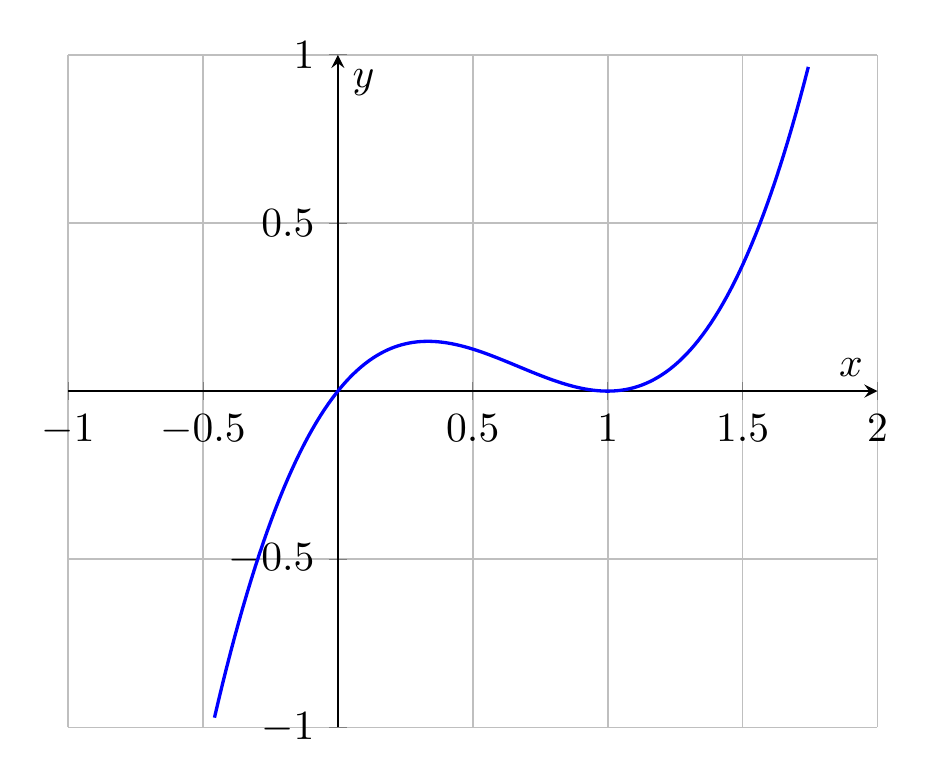
\begin{tikzpicture}[scale=1.5]
            \begin{axis}[
                axis lines=middle,
                grid=major,
                xmin=-1, xmax=2,
                ymin=-1, ymax=1,
                xlabel=$x$,
                ylabel=$y$,
                samples=200,
                restrict y to domain=-1:1
            ]
                \addplot[blue, thick, domain=-1:2]{x^3-2*x^2+x};
            \end{axis}
        \end{tikzpicture} 
    \end{image}
     %\xmalt sketch of the function $x^3-2x^2+x$.
    }
    \item $f(x)=x^2-8x^{\frac{1}{2}},\,\,\,\,\,\,\, (x\geq 0)$\\
    \textcolor{blue}{$f'(x)=2x-4x^{-\frac12}$\\
    $f'(x)=2x-\frac{4}{x^{1/2}}$\\
    $f'$ DNE when $x=0$\\
    $f'(x)=0$:\\
    $2x-\frac4{x^{1/2}}=0$\\
    $2x=\frac4{x^{1/2}}$\\
    $2x^{3/2}=4$\\
    $x^{3/2}=2$\\
    $x=\sqrt[3]{4}$\\
    \begin{tabular}{c|c|c}
       Interval  & $f'$ & $f$  \\ \hline
     $(0,\sqrt[3]{4})$ & - & decreasing \\
     $(\sqrt[3]{4},\infty)$ & + & increasing\\
    \end{tabular}\\
    $x=\sqrt[3]{4}$ is the location of a local minimum\\
    $f''(x)=2+2x^{-3/2}$\\
    $f''(x)=2+\frac{2}{x^{3/2}}$\\
    $f''$ DNE when $x=0$\\
    $f''(x)=0$:\\
    $2+\frac{2}{x^{3/2}}=0$\\
    $\frac{2}{x^{3/2}}=-2$
    $2=-2x^{3/2}$ has no solution.\\
    \begin{tabular}{c|c|c}
        Interval & $f''$ & $f$  \\ \hline
       $(0,\infty)$  & + & cc up \\
    \end{tabular}\\
    There is no inflection point.\\
    \begin{image} 
        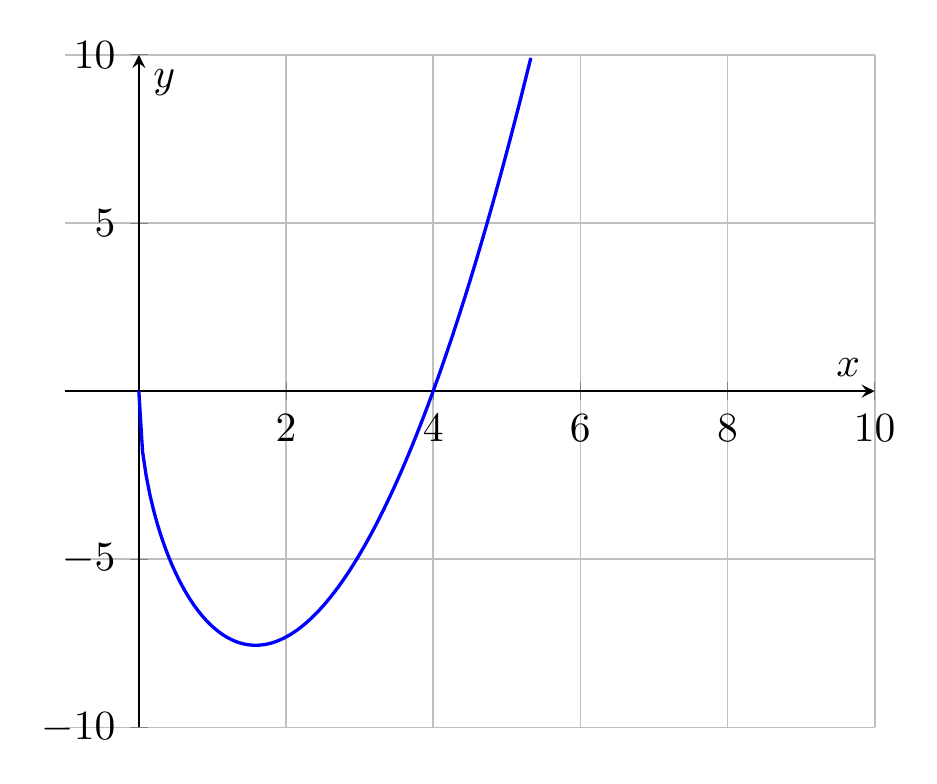
\begin{tikzpicture}[scale=1.5]
            \begin{axis}[
                axis lines=middle,
                grid=major,
                xmin=-1, xmax=10,
                ymin=-10, ymax=10,
                xlabel=$x$,
                ylabel=$y$,
                samples=200,
                restrict y to domain=-10:10
            ]
                \addplot[blue, thick, domain=0:10]{x^2-8*x^(1/2)};
            \end{axis}
        \end{tikzpicture}   
    \end{image}
    %\xmalt sketch of the function $x^2-8x^{\frac{1}{2}}$.
    }

    %\item $f(x)=x+\sin(x),\,\,\,\,\,\,\, x\in [0,2\pi]$
    \item $f(x)=(x^2-3)e^{-x}$ \\
    \textcolor{blue}{$f'(x)=(2x)(e^{-x})+(x^2-3)(-e^{-x})$\\
    $=e^{-x}(2x-x^2+3)$\\
    $f''(x)=e^{-x}(2-2x)-e^{-x}(2x-x^2+2)$\\
    $=e^{-x}(-2x+x^2)$\\
    \\
    $f'(x)=0$ when $e^{-x}(2x-x^2+2)=0$ or $e^{-x}(-x+3)(x+1)=0$, so $x=3$, $x=-1$ or $e^{-x}=0$ (which has no solution).\\
    $f'(x)$ DNE never\\
    \begin{tabular}{c|c|c}
        Interval & $f'$ $f$ \\ \hline
        $(-\infty,-1)$ & - & decreasing\\
        $(-1,3)$ & + & increasing \\
        $(3,\infty)$ & - & decreasing\\    
    \end{tabular}
    \\
    $f''(x)=0$ when $e^{-x}(-2x+x^2)=0$ or when $e^{-x}=0$ (no solution) or $x(-2+x)=0$, so $x=0$ and $x=2$.\\
    $f''(x)$ DNE never\\
    \begin{tabular}{c|c|c}
        Interval & $f''$ & $f$\\ \hline
        $(-\infty, 0)$ & + & cc up \\
        $(0,2)$ & - & cc down \\
        $(2,\infty)$ & + & cc up \\
    \end{tabular}
    \\
    $f(-1)=-2e$ \\
    $(-1,-2e)$ is a local min\\
    $f(3)=\frac{6}{e^3}$\\
    $(3,\frac{6}{e^3})$ is a local max
    $f(0)=3$\\
    $f(2)=\frac{1}{e^2}$\\
    $(0,3)$ and $(2,\frac{1}{e^2})$ are inflection points.\\
    \begin{image} 
        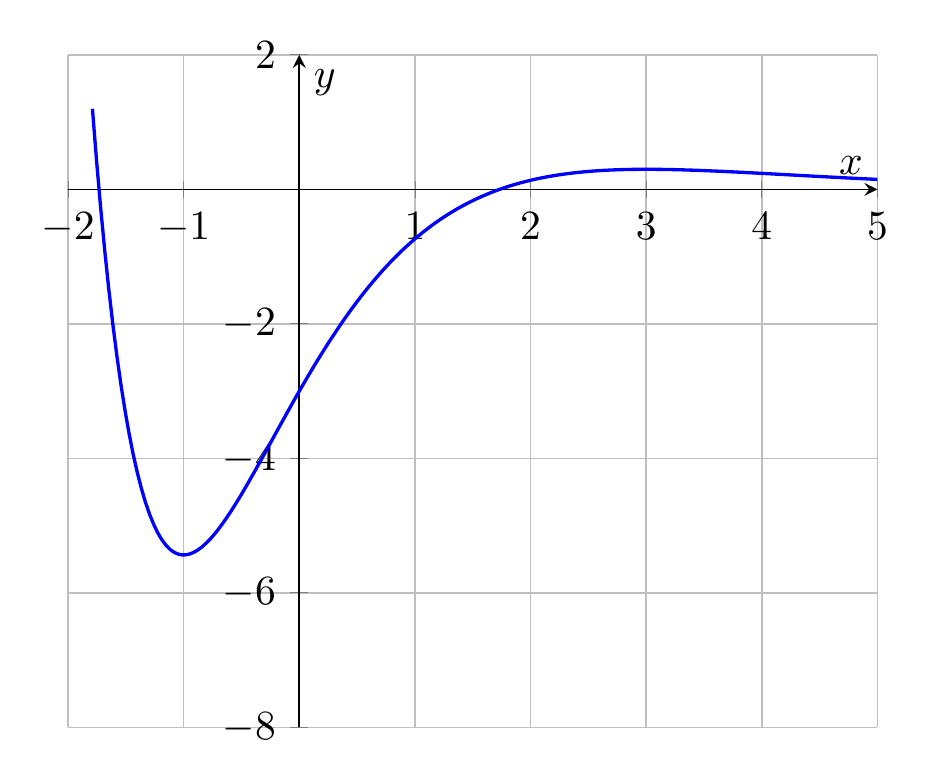
\begin{tikzpicture}[scale=1.5]
            \begin{axis}[
                axis lines=middle,
                grid=major,
                xmin=-2, xmax=5,
                ymin=-8, ymax=2,
                xlabel=$x$,
                ylabel=$y$,
                samples=200,
                restrict y to domain=-8:2
            ]
                \addplot[blue, thick, domain=-2:5]{(x^2-3)*exp(-x)};
            \end{axis}
        \end{tikzpicture}
    \end{image}
    %\xmalt sketch of the graph of $f(x)=e^{-x}(x^2-3)$.
    }

    \item $f(x)=\dfrac{x^3}{x+1}$
      \textcolor{blue}{$f'(x)=\dfrac{(x+1)(3x^2)-x^3}{(x+1)^2}=\dfrac{2x^3+3x^2}{(x+1)^2}$\\
    $f''(x)=\dfrac{(x+1)^2(6x^2+6x)-2(x+1)(2x^3+3x^2)}{(x+1)^4}$\\
    $=\dfrac{(x+1)\big((x+1)(6x^2+6x)-2(2x^3+3x^2)\big)}{(x+1)^4}$\\
    $=\dfrac{6x^3+6x^2+6x^2+6x-4x^3-6x^2}{(x+1)^3}$\\
    $=\dfrac{2x^3+6x^2+6x}{(x+1)^3}$\\
    $=\dfrac{2x(x^2+3x+3)}{(x+1)^3}$\\}
    \\
    \textcolor{blue}{
    $f'(x)=0$ when $2x^3+3x^2=0$ or $x^2(2x+3)=0$ so $x=0$ and $x=-\frac{3}{2}$\\
    $f'(x)$ DNE when $(x+1)^2=0$ or when $x=-1$.\\
    \begin{tabular}{c|c|c}
        Interval & $f'$ & $f$\\ \hline
       $(-\infty,-\frac32)$  & - & decreasing  \\
       $(-\frac32,-1)$ & + & increasing \\
       $(-1, 0)$ & + & increasing \\
       $(0,\infty)$ & + & increasing
    \end{tabular}}
    
    
    \textcolor{blue}{
    $f''(x)=0$ when $2x(x^2+3x+3)=0$ or when $x=0$ or $x^2+3x+3=0$.  This quadratic has no real roots\\
    $f''(x)$ DNE when $(x-1)^3=0$ or $x=-1$\\
    \begin{tabular}{c|c|c}
        Interval &  $f''$ & $f$ \\ \hline
        $(-\infty, -1)$ & + & concave up\\
        $(-1,0)$ & - & concave down\\
        $(0,\infty)$ & + & concave up
    \end{tabular}}
    \\
    \textcolor{blue}{
    $f(-\frac32)=\dfrac{(-\frac32)^3}{-\frac32+1}$\\
    $(-\frac32, \frac{27}{4})$ is a local min\\
    ($x=-1$ is not in the domain of the function, so it is not a critical point or inflection point) \\
    $f(0)=0$\\
    $(0,0)$ is an inflection point.\\}
     \begin{image} 
        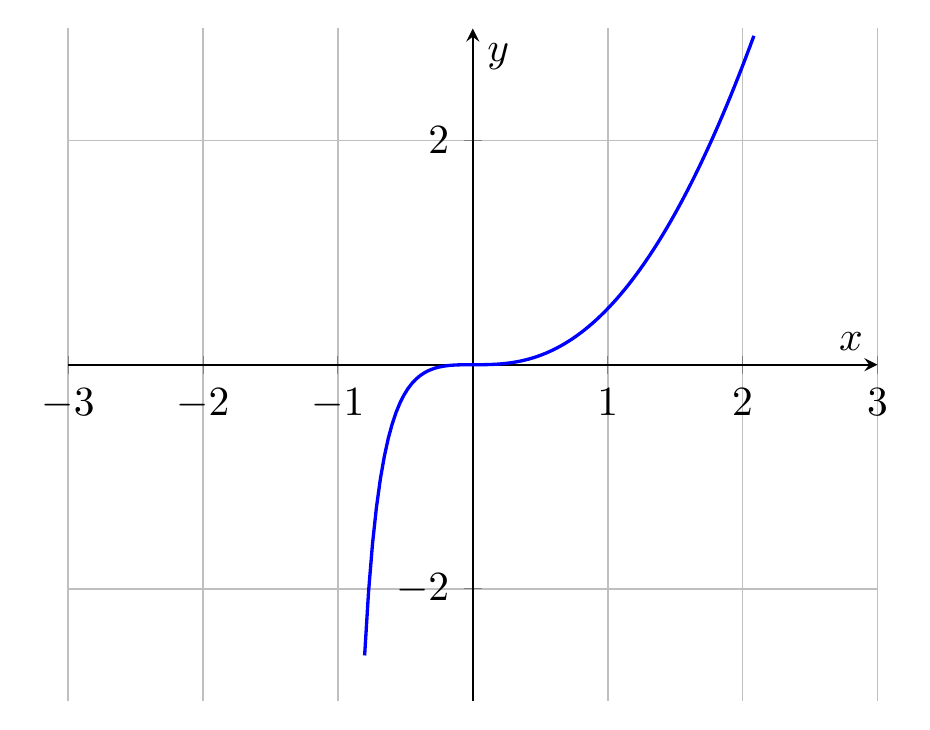
\begin{tikzpicture}[scale=1.5]
            \begin{axis}[
                axis lines=middle,
                grid=major,
                xmin=-3, xmax=3,
                ymin=-3, ymax=3,
                xlabel=$x$,
                ylabel=$y$,
                samples=200,
                restrict y to domain=-3:3
            ]
                \addplot[blue, thick, domain=-2.9:2.9]{x^3/(x+1)};
            \end{axis}
        \end{tikzpicture}
    \end{image}
        %\xmalt sketch of the function $\dfrac{x^3}{x+1 }$.
    
    
\end{enumerate}
\end{exercise}





\end{document}
